\NextFile{SystemRequirements.html}
\chapter{System Requirements and performance}

\authorsOfDoc{Marcel Rieser, Johan W. Joubert}

\bigskip

%%\begin{chapter-intro}
%%Some chapter intro.
%%\end{chapter-intro}

\section{Software}

MATSim runs on any machine that has the \href{http://java.sun.com/javase/downloads/index.jsp}{Java Platform, Standard Edition} (SE) 6 or newer installed (commonly referred to as ``Java 6" or newer).

\section{Hardware}

Smaller  scenarios (e.g. the examples included in the tutorials, 5\%- or  10\%-samples of large scenarios) can be run on common desktop or laptop  computers.

To simulate large scenarios (several hundreds of  thousands of agents, networks with ten-thousands of links and nodes),  high end computers with a large amount of memory (RAM) may be required  to keep the agents' data in memory. The description of agents' plans and  the simulation output can take several Gigabytes of hard disk space. To  store the data for several scenarios and / or output of simulation  runs, large amounts of disk space may thus be needed. MATSim can read  and write compressed files to reduce the amount of required disk space,  but this aspect still shouldn't be underestimated. MATSim can make use  of multiple CPUs or CPU cores that share common memory (``shared memory  machine'') during the replanning-phase.

Running large scenarios for  a high number of iterations can take several hours, up to a few days.  Thus it may be advisable to have a dedicated machine running MATSim if  you plan to simulate many different scenarios.

\subsection{Recommendations}
\begin{itemize}
	\item To try MATSim out:
\\Any modern laptop or desktop computer with 1GB RAM and 500MB free disk space should be suitable.
	\item To run a large scenario (100 000+ agents, networks with 50 000+ links): 
\\A high-end desktop computer with at least 4GB RAM and 200 GB free disk space.
	\item To run many large scenarios, so they can be compared against each other: 
\\Multiple high-end desktop computers or servers with at least 4GB RAM that share a common storage disk (at least 1TB).
\end{itemize}

The  high numbers for free disk space result from the fact that the  simulation writes quite a lot of data to the disk during a run. For  analysis, usually only the last version of the data is required, and  data from earlier iterations can be deleted, freeing space up again.

\subsection{What we use}

Currently,  we simulate most of our scenarios on machines with 16 or 32 GB RAM,  having 2 dual- or quad-core processors. The amount of memory allows us to run 2  scenarios at the same time on the machines. A \href{http://en.wikipedia.org/wiki/RAID}{RAID}  array is used as storage backend, offering about 4 TB of hard disk  space. This huge disk space is able to store the results of hundreds of  simulations and will suit us for the next few years. Computers and RAID  are regular components used in data centers, nowadays available at moderate prices.

\section{Benchmarks}

There are a few benchmark exercises you can consider in MATSim.

\subsection{Standard MATSim benchmarks}
\subsubsection{Overview}
The performance of MATSim depends on a lot of different factors:
\begin{itemize}
\item CPU-speed (although by far not always the limiting factor!)
\item Memory-Bus / -Controller (we're moving huge amounts of memory, the faster the better)
\item Java Virtual Machine (JVM 1.7 is usually faster than JVM 1.6)%%, {\color{red} and we are now (September 2014) officially on Java 1.7}.
\item File system (local Hard drive vs. RAID vs. NFS vs \ldots)
\end{itemize}
To get a better understanding, under which circumstances MATSim performs best, we created a simple benchmark (performance test) that runs 20 iterations of a sample scenario with different settings. If you run the benchmark on your machine, we would be happy if you could send us your results.

\subsubsection{Download and installation}
Download the following zip-file: \href{http://matsim.org/files/benchmark/benchmark.zip}{benchmark.zip}{[35MB]}. Unzip the downloaded file.

\subsubsection{Running the benchmark}
On the command line, run the following:
\begin{lstlisting}{language=xml}
java -Xmx500m -jar Benchmark.jar
\end{lstlisting}
This will generate a directory output with some files in it from the run. The test will usually run between 25 and 40 minutes. The benchmark requires Java 1.5 or newer and 150MB free disk space. If you want to re-run the benchmark, rename or delete the \texttt{./output/} directory and run the test again.

\subsubsection{Submitting benchmark results}
Please send an email to \texttt{benchmark AT matsim DOT org} containing:
\begin{itemize}
\item the file \texttt{output/stopwatch.txt}
\item the file \texttt{output/logfile.log}
\item a description of your benchmark environment, including:
\begin{itemize}
\item vendor of machine (e.g. Sun, Dell, Apple, etc.)
\item processor-type (vendor (AMD, Intel, etc.), model-number, clock-speed, cache-size, number of processors and cores, \ldots)
\item memory (bus-speed, memory-controller, etc.)
\item storage system (rpm, cache size, \ldots, type: e.g. local hard drive, RAID, \ldots)
\item operation system
\item java virtual machine
\item any other information you think might be of interest to us
\end{itemize}
\end{itemize}

We collected some results and did a short analysis on them. Have a look at the results in the next section. If you want your results included as well or have some interesting findings yourself, please submit us your benchmark results.

\subsection{MATSim benchmark results}
The benchmark contains parts of the code running in parallel (the replanning part, using 4 threads) and other parts running single-threaded.

\subsubsection{Speed comparison}
The benchmark was run on some of our production servers with different versions of Java Virtual Machines. The servers have 2 Single-Core ``AMD Opteron Processor 248'' running at 2.2 GHz (date of purchase: fall 2004, so they have to be considered as \emph{old}). The Java Virtual Machines tested were:

\begin{description}
\item[IBM Java 5 64bit]\quad The default Java 5 version on the servers. The JVM identified itself as \texttt{J2RE 1.5.0 IBM J9 2.3 Linux amd64-64 j9vmxa6423ifx-20080811}
\item[Sun 6u5 64bit]\quad The default Java 6 version on the servers, identifying itself as \texttt{1.6.0\_05; Sun Microsystems Inc.; mixed mode; 64-bit}
\item[Sun 5u19 64bit]\quad The latest (as of writing this text) Java 5 version from Sun, Java 5 update 19 64-bit.
\item[Sun 5u19 32bit]\quad The latest Java 5 version from Sun, Java 5 update 19 32-bit.
\item[Sun 6u14 64bit]\quad The latest Java 6 version from Sun, Java 6 update 14 64-bit.
\item[Sun 6u14 32bit]\quad The latest Java 6 version from Sun, Java 6 update 14 32-bit.
\item[Sun 6u14 64bit COP]\quad Sun's Java 6 update 14 64-bit, started with the extra argument \texttt{-XX:+UseCompressedOops}. Compressed Object Pointers should "improve performance of the 64-bit JRE when the Java object heap is less than 32 gigabytes in size" (see \href{http://java.sun.com/javase/6/webnotes/6u14.html}{Java SE 6 Update 14 Release Notes}). As an additional advantage, memory consumption should also be a bit lower when using only 32bits for object pointers.
\item[Sun 6u14 64bit COP + AO]\quad Sun's Java 6 update 14 64-bit, started with the extra argument \texttt{-XX:+UseCompressedOops -XX:AggressiveOpts}. In addition to using Compressed Object Pointers, also try out the new \emph{experimental implementation} of \texttt{java.util.TreeMap} that can improve the performance as MATSim makes heavy use of TreeMaps (although not necessarily that often iterating over them)
\item[Sun 6u14 32bit AO]\quad Sun's Java 6 update 14 32-bit, started with the extra argument \texttt{-XX:AggressiveOpts}. Just for comparison, also start the 32-bit version of the JVM with the aggressive optimization option.
\end{description}

The shown number in Figure~\ref{fig:Benchmark01} are the average of two runs of the benchmark for each configuration (Yeah, two isn't that big a sample, we know... but it should still be valid to demonstrate some findings).
\begin{figure}[h]
\centering
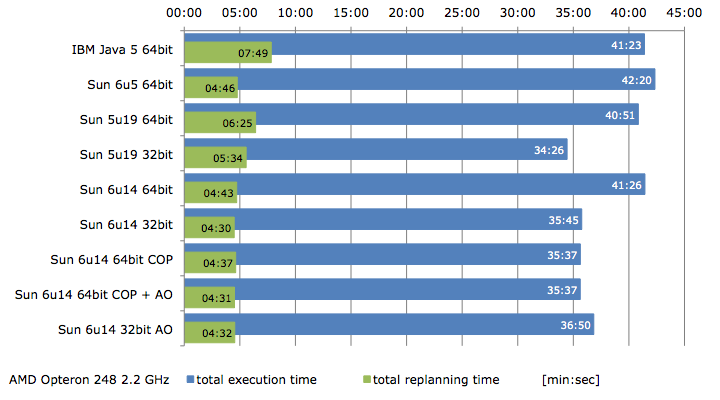
\includegraphics[width=0.75\linewidth]{figures/benchmarks/benchmark1}
\caption{The average of two runs of the benchmark for each configuration.}
\label{fig:Benchmark01}
\end{figure}
What can be observed is the huge difference of execution time in general between 32-bit and 64-bit versions of the virtual machines. The \emph{compressed object pointers} (COP) feature of Suns JVM 6u14 seems to compensate for this nicely, making the 64-bit version about the same speed than the 32-bit version. The aggressive optimization options (AO) on the other hand doesn't seem to influence the performance of MATSim drastically.

While the difference between Suns Java 5 and Java 6 versions in the total execution time seem more or less random, there seems to be a performance improvement for the multithreaded replanning part by changing from Java 5 to Java 6. Interestingly, despite IBM's worse multithreaded performance, it is able to catch up in the single-threaded parts to come in with a similar total execution time than Sun's 64-bit JVMs.

The benchmark was also run on other server machines:

\begin{itemize}
\item Servers with two Dual-Core AMD Opteron 2222 processors, running at 3.0 GHz; date of purchase winter 2007/2008 (very similar architecture than the previously tested AMD Opteron 248 systems, just \emph{newer} with higher clocked CPU).
\item Servers with Intel Xeon X5355 Quad-Core processors, clocked at 2.66 GHz, 8 MB L2 cache, built with 65 nm technology.
\item Servers with Intel Xeon E5430 Quad-Core processors, clocked at 2.66 GHz, 12 MB L2 cache, built with 45 nm technology.
\item Servers with Intel Xeon E5530 Quad-Core processors, clocked at 2.4 GHz, 8 MB L3 cache, 45 nm technology, Nehalem architecture.
\item Servers with Intel Xeon E7540 Hex-Core processors, clocked at 2.0 GHz, 18 MB L3 cache, 45 nm technology, Nehalem architecture, DDR3 RAM.
\end{itemize}
Comparing (in Figure~\ref{fig:Benchmark02}) the AMD servers running at 2.2 GHz and 3.0 GHz, the most obvious difference is the time for the replanning, explainable by the different number of cores the machines have. 
\begin{figure}[h]
\centering
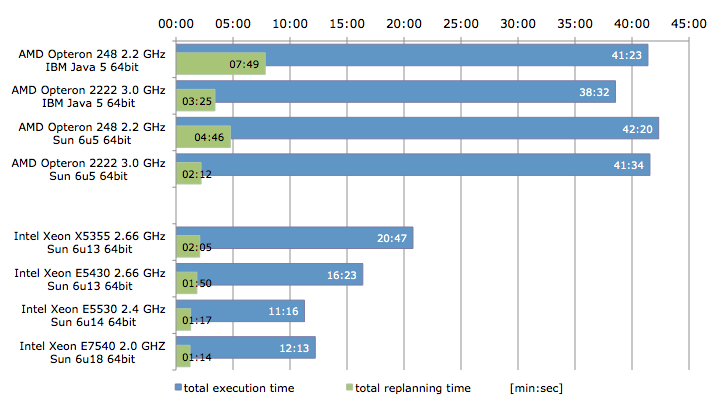
\includegraphics[width=0.75\linewidth]{figures/benchmarks/benchmark2}
\caption{The average of two runs of the benchmark for different servers.}
\label{fig:Benchmark02}
\end{figure}
Interestingly, the remaining execution time didn't really improve by the change in CPU speed, leading to the guess that the performance of the memory controller or the memory bus is limiting the speed of MATSim (both AMD servers seem to have a front side bus of 1000 MHz).

The Intel servers were massively faster than the AMD machines. We do not yet know if it's the different memory controller, faster memory bus, or if Sun's JDK is just more optimized for Intel processors. Anyway, the difference is striking. And each newer generation of Intel processors seems to deliver a real performance upgrade, even when running at a lower clock-speed.

At last, the benchmark was also run on some of our laptop machines: An Apple MacBook Pro with a Intel Core 2 Duo processor clocked at 2.33 GHz (model from fall 2006), running Mac OS X 10.5.7, and an IBM/Lenovo Laptop with the same Intel Core 2 Duo processor, 2.33 GHz, running a Gentoo 64-bit Linux (Kernel 2.6.28). Both laptops have a front side bus of 667 MHz, so from a technical view point they are very similar.

On the Apple MacBook Pro, the following Java Virtual Machines were used:

\begin{description}
\item[Apple JVM 5u16 32bit]\quad The default Java 5 version on Mac OS provided by Apple.
\item[Apple JVM 6u7 64bit]\quad The default Java 6 version on Mac OS provided by Apple.
\item[Soylatte 6u3 32bit]\quad An early port of OpenJDK 6, identifying itself as \texttt{1.6.0\_03-p3; Sun Microsystems Inc.; mixed mode; 32-bit}, provided by \href{http://landonf.bikemonkey.org/static/soylatte/}{Landon Fuller}.
\end{description}
On the Lenovo Laptop, an OpenJDK 6u0 64-bit JVM was used.
\begin{figure}[h]
\centering
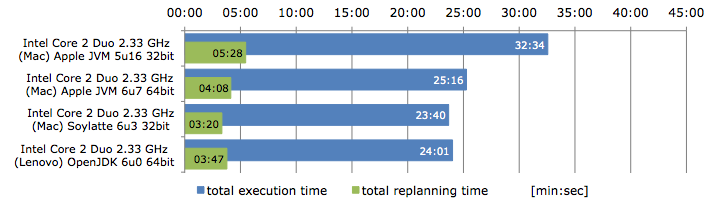
\includegraphics[width=0.75\linewidth]{figures/benchmarks/benchmark3}
\caption{The average of two runs of the benchmark for laptops.}
\label{fig:Benchmark03}
\end{figure}
Surprisingly, Apple pulled the trick to make their 64-bit Java 6 a lot faster than the older 32-bit Java 5—well, it could also mean that their Java 5 offering was just very slow\ldots The Mac-port of OpenJDK 6 (\emph{Soylatte}) is even a bit faster, but that may be likely due to the difference between 64-bit and 32-bit.

Are you able to run the MATSim benchmark even faster? Please tell us so! We're very interested in your benchmark results.

\subsubsection{Memory usage comparison}
MATSim writes out information about memory usage from time to time into the logfile. Plotting this information gives a jagged line running from left to right. Heights and lows in the plot can be explained with the Java Garbage Collector, only freeing up the memory from time to time. Still, one can guess the absolute minimum of memory required by MATSim by looking at the lower parts of the curve (that's then when a Garbage Collection just ran, showing all the memory that could not be collected).

Comparing the memory consumption in Sun's (currently) latest Java VM version holds no real surprises.
\begin{figure}[h]
\centering
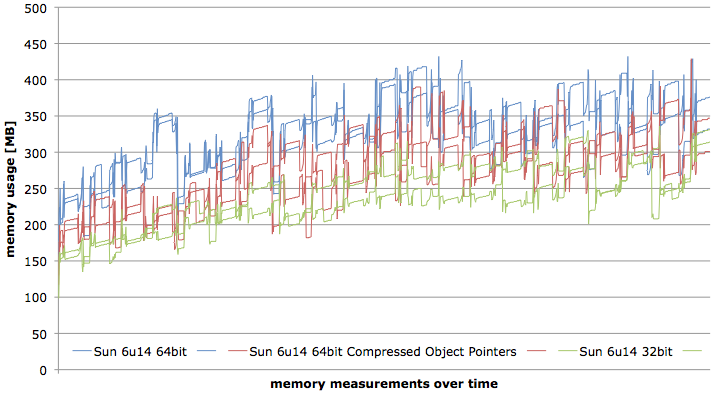
\includegraphics[width=0.75\linewidth]{figures/benchmarks/benchmark_memory}
\caption{Memory usage over iterations.}
\label{fig:Benchmark04}
\end{figure}

It can be clearly seen that the 64-bit JVM uses the largest amount of memory, due to the fact that each object pointer takes up 8 bytes. The 32-bit JVM uses the least memory. The 64-bit JVM with compressed object pointers seems to lie somewhere in between—although I would have expected it to be comparable to the 32-bit JVM, it seems that it still uses a bit more memory for unknown reasons. Anyway, it comes in handy to know that one can load now larger scenarios on a 32GB (or less) machine. The memory savings, compared to a 64-bit JVM without compressed object pointers, should be even bigger the larger the scenario is or the more details the simulated network has, so this feature really looks promising.
 
So, by how much can you improve your MATSim simulation's performance?

\section{Speeding up your own MATSim runs}
There are a few things you can try to speed up your simulation runs. The following hints are not in any specific order.%% {\color{red}(are they?)}.

\subsection{Use an up-to-date Java version}
Java 7 usually performs better than Java 6.

\subsection{Use compressed object pointers in 64-bit JVM}

Since Sun Java 6, Update 14, if you use a 64-bit JVM and use at most 32 GB of RAM, start Sun's Java virtual machine with the argument 
\begin{lstlisting}{language=xml}
-XX:+UseCompressedOops
\end{lstlisting}
This reduces the size of object pointers to 32 bit, making many pointer operations a lot faster than when they were 64 bit long, while still supporting heap sizes larger than 2 GB (what a regular 32-bit JVM would do). See the \href{http://www.oracle.com/technetwork/java/javase/6u14-137039.html}{Java SE 6 Update 14 Release Notes} for more details. In addition, we observed notable speed-ups in the region of 10\% in the run time of MATSim. Since Java SE 6 Update 23 and in Java 7, this option is enabled by default.

\subsection{Parallelization}
When running a MATSim simulation, unused cores can be utilized to make the simulation faster. There are now three ways to improve performance using parallelization, and each can be switched on or off separately.

\subsubsection{Event handling}\label{sec:ParallelEventsHandling}
The event handler which is used by default, is running in the same thread as the simulation. For this reason, you can switch on parallel event handling by adding the \texttt{parallelEventHandling} module to the MATSim \texttt{Config} XML file as follows:
\begin{lstlisting}{language=xml}
<module name="parallelEventHandling">
    <param name="numberOfThreads" value="1" />
</module>
\end{lstlisting}
The only required parameter in this module is \texttt{numberOfThreads}. The value of this parameter specifies how many threads (cores) should be assigned to handling events.

There is an additional optional parameter \texttt{estimatedNumberOfEvents}, which can be optimized to your simulation resulting in slightly faster runs. But its usage requires an estimate of the number of events which will occur in one iteration.
\begin{lstlisting}{language=xml}
<param name="estimatedNumberOfEvents" value="5000000" />
\end{lstlisting}
The following are some hints to consider and pitfalls to avoid:
\begin{itemize}
\item Don't make any  assumptions on the order, in which the handlers are executed (as they are executed in parallel).
\item Don't write the data in one handler and read that data in a different handler. Although this is possible, special care is required as synchronization between threads is needed for this. Furthermore this could lead to a degradation of the speed up.
\item There is no point in using parallel event handling, if you have just one core available on your machine.
\item Always make sure, that one thread is needed for the single cpu simulation. This means, if you have 4 cores, you can set the parameter 'numberOfThreads' to maximum 3.
\item If 2 handlers have been added to the simulation, then there is no point in assigning 3 threads to parameter \texttt{numberOfThreads}, because it won't make the simulation faster (but rather could slow it down in some cases).
\item The number of handlers can be bigger than \texttt{numberOfThreads}. In this case automatically if possible, each thread is assigned the same number of handlers. 
\item If the simulation is quite slow (compared to event handling), you won't be able to make full use of parallel event handling.
\end{itemize} 
The actual speed up you get depends on many factors, especially on those in the aforementioned hints and pitfalls. Experiments on a 16 core machine with different numbers of handlers have shown that the parallel event handler can reduce the simulation time with a very low overhead. Some Java specific implementation aspects of \emph{JDEQSim} and the \texttt{parallelEventHandling} module are described in the paper by Waraich, R., D. Charypar, M. Balmer and K.W. Axhausen (2009) Performance improvements for large scale traffic simulation in MATSim, paper presented at the 9th Swiss Transport Research Conference, Ascona, September 2009. This paper can be downloaded \href{http://www.ivt.ethz.ch/vpl/publications/reports/ab565.pdf}{here}. 

\subsubsection{Mobility simulation}\label{sec:ParallelQsim}
\authorsOfCode{C. Dobler, IVT}
\maintainers{C. Dobler, IVT}

There is a parallel version of the qsim. Analysis of performance and structure of (non parallel) qsim shows:
\begin{itemize}
\item Simulation of movement on links and over nodes is most time consuming.
\item Within a timestep actions on nodes and links can be simulated on parallel threads with low additional synchronization effort.
\end{itemize}

The parallel qsim is based on the existing qsim and can be used by just adding a new parameter to a scenario configuration file (see ). First performance measurements show promising results, and a working paper will be published in Q2 2010. A structural description of the parallel qsim is shown in Figure~\ref{fig:ParallelQsim}.
\begin{figure}[htp]
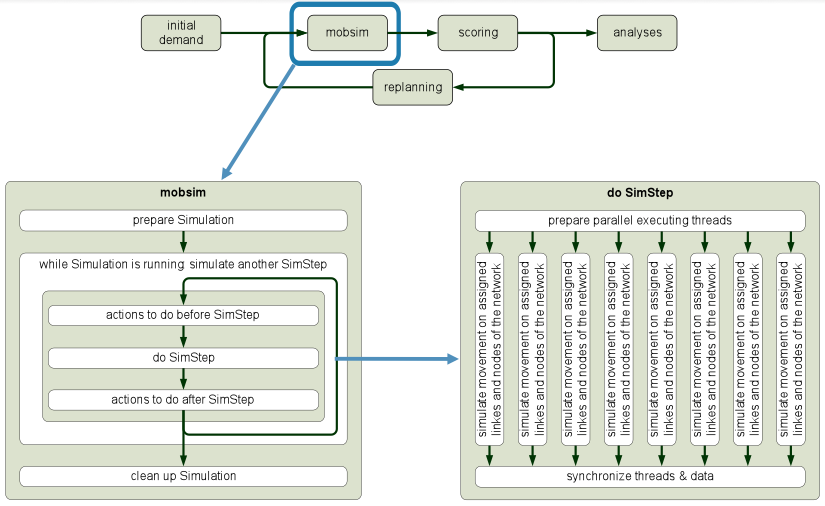
\includegraphics[width=\textwidth]{figures/qsimParallel/parallelqsim.png}
\caption{Design of the parallel qsim.}\label{fig:ParallelQsim}
\end{figure}

To activate it, ensure that a \texttt{qsim} module is added to the config XML file of MATSim, and set the \texttt{numberOfThreads} parameter as follows:
\begin{lstlisting}{language=xml}
<module name="qsim">
   ...
   <param name="numberOfThreads" value="5"/>
</module>
\end{lstlisting}
or however many number of threads you want to use. An unlimited number of threads will \emph{not} make your simulation run infinitely fast. A performance \emph{decrease} can actually occur, depending on the scenario size. Refer to Christoph Dobler's thesis (Chapter 5) for a complete discussing in this regard. Figure~\ref{fig:QsimPerformance} shows an estimation of the (optimal) number of threads required for a given scenario size (expressed as number of events generated).
\begin{figure}[h]
\centering
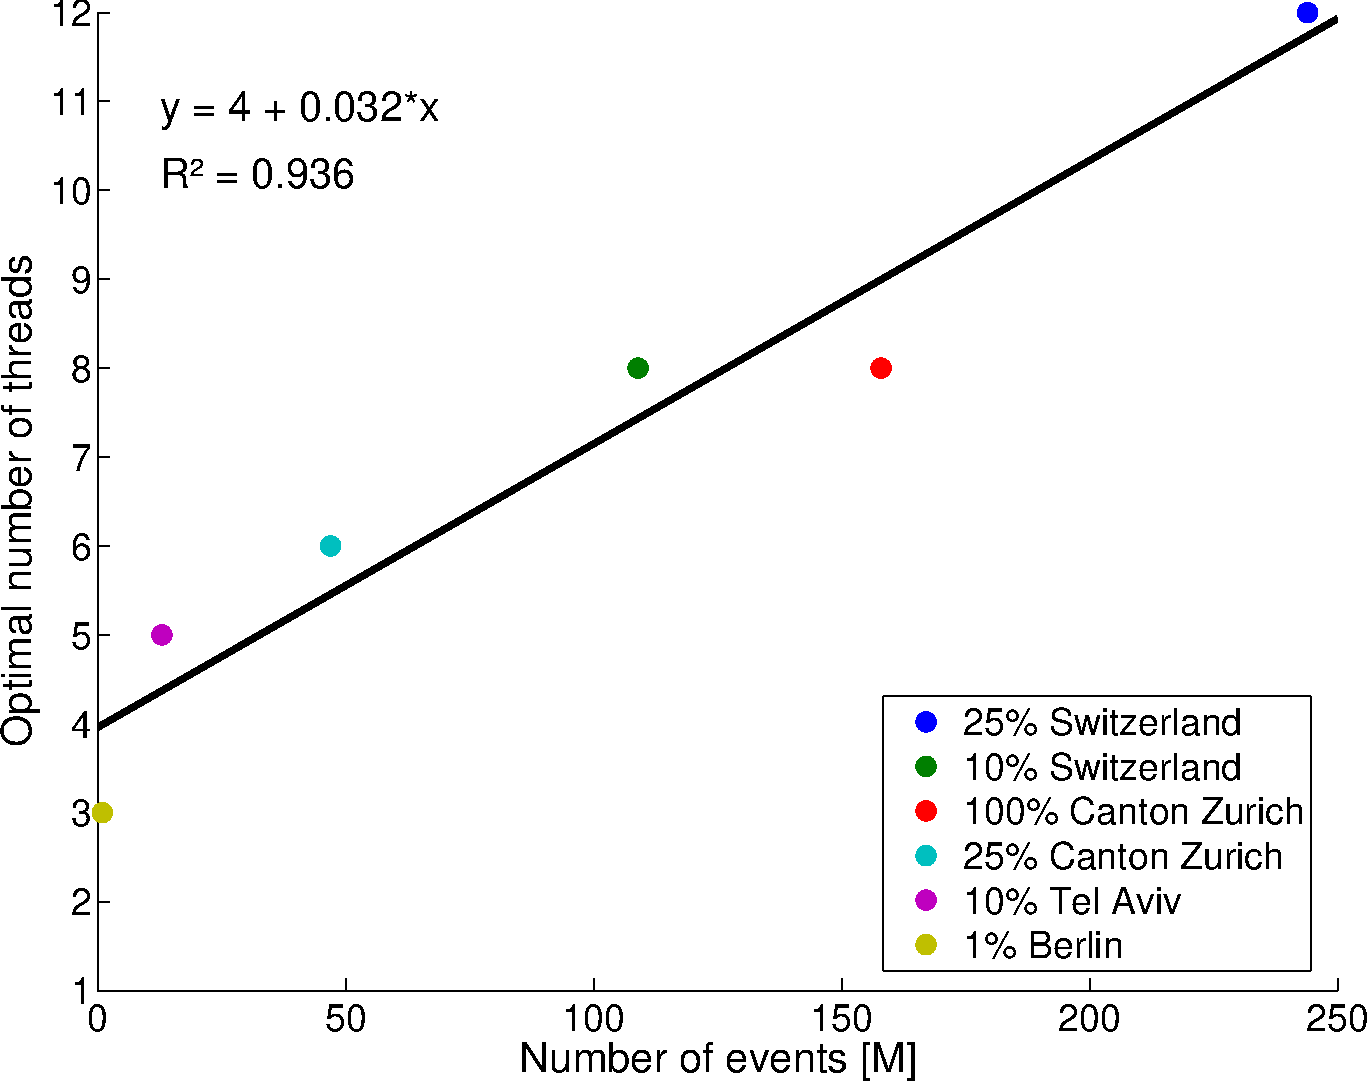
\includegraphics[width=0.6\linewidth]{figures/benchmarks/EventsVsSpeedUp}
\caption{Estimated number of threads to use for a given scenario size.} 
\label{fig:QsimPerformance}
\label{figureLabel}
\end{figure}

Dobler, C. (2013). Travel behaviour modelling for scenarios with exceptional events --- methods and implementations, Dissertation, IVT, ETH Zurich, Zurich. Available online \href{http://e-collection.library.ethz.ch/view/eth:7633}{here}.

\subsubsection{Replanning}
To set the simulation to parallelize the replanning phase, the following parameter must be set the the \texttt{global} module of the config XML file:
\begin{lstlisting}{language=xml}
<module name="global">
  ...
  <param name="numberOfThreads" value="8" />
</module>
\end{lstlisting}

\subsection{Limit the writing of events}
Writing the simulation events to files in each iteration not only consumes a lot of disk space, but also a considerable amount of time. Add the following parameter to your configuration to restrict writing events to certain iterations:
\begin{lstlisting}{language=xml}
<module name="controler">
  ...
  <param name="writeEventsInterval" value="10" />
</module>
\end{lstlisting}

\subsection{Use faster routing algorithms}
By default, MATSim uses a routing algorithm based on Dijkstra's shortest path algorithm. But MATSim also includes a faster routing algorithm, based on the A$^{\star}$ algorithm with landmarks. To use this routing algorithm, add the following configuration parameter to your configuration file:
\begin{lstlisting}{language=xml}
<module name="controler">
  ...
  <param name="routingAlgorithmType" value="AStarLandmarks" />
</module>
\end{lstlisting}

\subsection{Comparing parallelisation options}
The following shows two different benchmarks using jdeqsim (Section~\ref{sec:Jdeqsim}), parallel events handling (Section~\ref{sec:ParallelEventsHandling}), or both. The first benchmark, Figure~\ref{fig:JdeqsimTime}, uses the ivtch-osm network (approximately 60,000 links), while the second one, Figure~\ref{fig:JdeqsimTime-navteq}, uses a navteq network with much more links.

\subsubsection{QueueSim versus JDEQSim using parallel events handling}
Zrh 10\%, ivtch-osm network; computing times per iteration (computer = cluster4 = 2x ``Dual-Core AMD Opteron Processor 2222'', 3.0 GHz, 1000 MHz FSB).  Runs 669, 676, 678, 679
\begin{figure}[h]
\centering
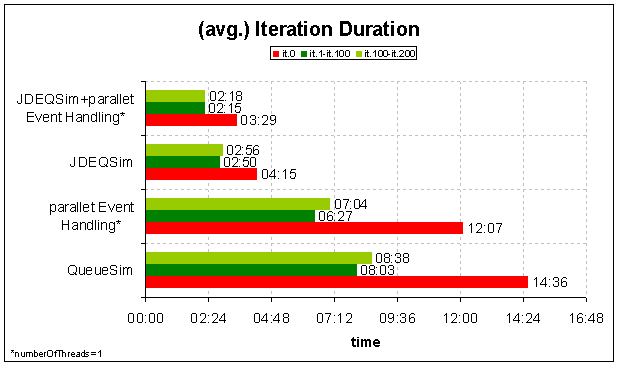
\includegraphics[width=0.75\linewidth]{figures/benchmarks/jdeqsimtime}
\caption{Using the ivtch-osm network.}
\label{fig:JdeqsimTime}
\end{figure}

Computing times per Iterations.  Scenario = navteq network of Switzerland; computer = cluster4 = servers with 2x ``Dual-Core AMD Opteron Processor 2222'', 3.0 GHz, 1000 MHz FSB.
\begin{figure}[h]
\centering
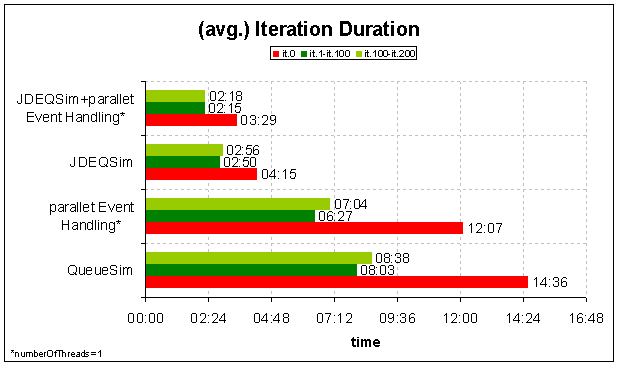
\includegraphics[width=0.75\linewidth]{figures/benchmarks/jdeqsimtime}
\caption{Using the ivtch-osm network.}
\label{fig:JdeqsimTime-navteq}
\end{figure}

